\documentclass[12pt,letterpaper]{exam}
\usepackage[lmargin=1in,rmargin=1in,tmargin=1in,bmargin=1in]{geometry}
\usepackage{../style/exams}

% -------------------
% Course & Exam Information
% -------------------
\newcommand{\course}{MAT 108: Exam 2}
\renewcommand{\term}{Spring -- 2022}
\newcommand{\examdate}{04/13/2022}
\newcommand{\timelimit}{85 Minutes}

\setbool{hideans}{true} % Student: True; Instructor: False

% -------------------
% Content
% -------------------
\begin{document}

\examtitle
\instructions{Write your name on the appropriate line on the exam cover sheet. This exam contains \numpages\ pages (including this cover page) and \numquestions\ questions. Check that you have every page of the exam. Answer the questions in the spaces provided on the question sheets. Be sure to answer every part of each question and show all your work. If you run out of room for an answer, continue on the back of the page --- being sure to indicate the problem number.} 
\scores
\bottomline
\newpage

% ---------
% Questions
% ---------
\begin{questions}

% Question 1
\newpage
\question Consider the function $f(x, y)= 3x - 2y$ on the `crooked house' feasible set shown below. 

	\[
	\fbox{
	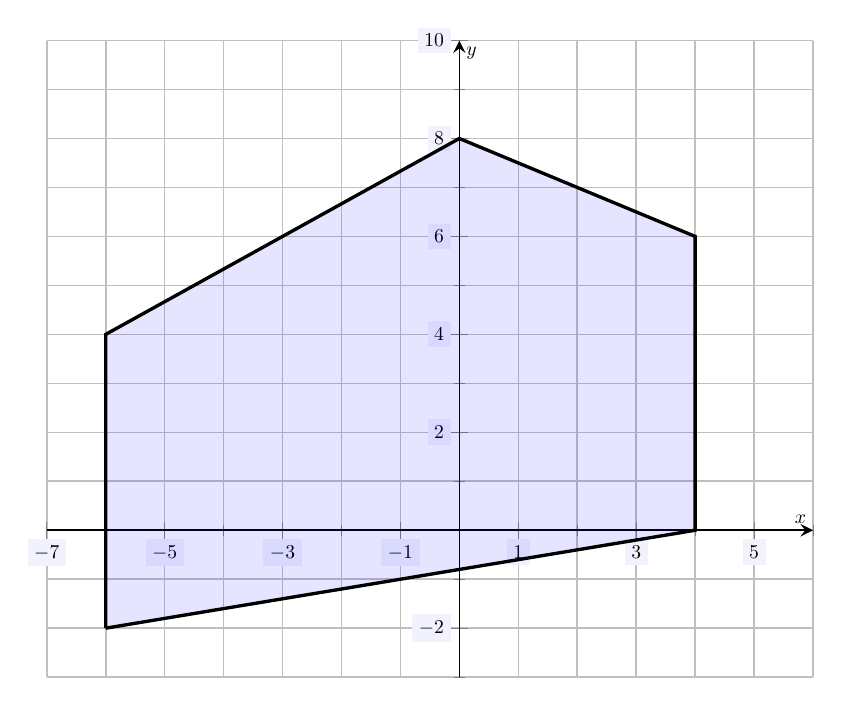
\begin{tikzpicture}[scale=1.42,every node/.style={scale=0.5}]
	\begin{axis}[
	grid=both,
	axis lines=middle,
	ticklabel style={fill=blue!5!white},
	xmin= -7, xmax=6,
	ymin= -3, ymax=10,
	xtick={-7,-5,...,7},
	ytick={-2,0,...,10},
	minor tick = {-10,-9,...,10},
	xlabel=\(x\),ylabel=\(y\),
	]
	\draw[line width=0.01cm,fill= blue,opacity=0.1] (-6,-2) -- (-6,4) -- (0,8) -- (4,6) -- (4,0) -- (-6,-2);
	\draw[line width=0.03cm] (-6,-2) -- (-6,4) -- (0,8) -- (4,6) -- (4,0) -- (-6,-2);
	\end{axis}
	\end{tikzpicture}
	}
	\] \pspace

\begin{parts}
\part[3] Explain why the Fundamental Theorem of Linear Programming applies to the function $f(x, y)$ on the feasible set shown above. \pvspace{3cm}
\part[7] Use the Fundamental Theorem of Linear Programming to find $\max f(x, y)$ and $\min f(x, y)$ on the feasible set shown above. 
\end{parts}



% Question 2
\newpage
\question[10] Find the initial simplex tableau for the linear programming problem shown below.
	\[
	\max z= 3x_1 - 5x_2 + 2x_3
	\]
	\[
	\left\{
	\begin{aligned}
	x_1 + 7x_2 - 3x_3 &\leq 10 \\
	2x_1 + 10x_3 &\leq 12 \\
	x_1 - x_2 + 5x_3 &\leq 7 \\
	x_1 - 4x_2 - 9x_3 &\geq -8
	\end{aligned} \right.
	\]
	\[
	x_1,\, x_2,\, x_3 \geq 0
	\]



% Question 3
\newpage
\question Below is the initial simplex tableau associated to a standard maximization problem. 
	\begin{table}[!ht]
	\centering
	\begin{tabular}{rrrrr|r}
	$2$ & $3$ & $1$ & $0$ & $0$ & $20$ \\
	$-1$ & $7$ & $0$ & $1$ & $0$ & $15$ \\
	$4$ & $1$ & $0$ & $0$ & $1$ & $30$ \\ \hline
	$9$ & $-5$ & $0$ & $0$ & $0$ & $0$ 
	\end{tabular}
	\end{table}

\begin{parts}
\part[1] How many inequalities were in the original problem? \vfill
\part[1] How many slack variables are there? \vfill
\part[1] How many decision variables are there? \vfill
\part[3] If one were to perform the simplex algorithm, circle the initial pivot position. \vfill
\part[4] Write the original maximization problem. \pvspace{3cm}\vfill
\end{parts}



% Question 4
\newpage
\question[10] Below is the final simplex tableau from the simplex algorithm used to solve a standard maximization problem. Find the solution along with the maximum value. Be sure to indicate the value of all variables involved. 
	\begin{table}[!ht]
	\centering
	\begin{tabular}{rrrrrrr|r}
	$0$ & $1$ & $-1.21$ & $0.05$ & $0.21$ & $0$ & $-0.05$ & $5.26$ \\
	$0$ & $0$ & $3.66$ & $16.21$ & $0.34$ & $1$ & $0.29$ & $321.05$ \\
	$1$ & $0$ & $0.82$ & $0.42$ & $0.18$ & $0$ & $0.08$ & $42.11$ \\ \hline
	$0$ & $0$ & $29.44$ & $99.39$ & $35.56$ & $0$ & $2.21$ & $4218.95$ \\
	\end{tabular}
	\end{table}



% Question 5
\newpage
\question[10] Below is a linear programming minimization problem. Find the associated dual problem. 
	\[
	\min w= 5x_1 + 4x_2
	\]
	\[
	\left\{
	\begin{aligned}
	4x_1 - x_2 &\geq 8 \\
	x_1 + 5x_2&\leq -12
	\end{aligned} \right.
	\]
	\[
	x_1,\, x_2 \geq 0
	\]
	


% Question 6
\newpage
\question Sal Ami wants to start offering weekly classes on fancy party hosting to stir up business for his delicatessen. To pay for some of the additions he will make to his shop, he takes out a \$2,500 loan from the bank and is charged a 5.8\% discount on the 6-month loan. \pspace

\begin{parts}
\part[3] What is the discount on the loan? \vfill
\part[2] What are the maturity and proceeds? \vfill
\part[2] What is Ami's effective interest rate? \vfill
\part[3] How much does Sal pay on the loan in total? \vfill
\end{parts}



% Question 7
\newpage
\question Bill Goulding is saving to purchase his dream food truck---Lord of the Fries. He places \$9,700 in an account which earns 6.1\% annual interest, compounded monthly. \pspace 
	
\begin{parts}
\part[3] How much is in this account after 7~years? \vfill
\part[4] How long until this account has \$20,000? \vfill
\part[3] What is the effective yearly interest rate for this account? \vfill
\end{parts}



% Question 8
\newpage
\question  Lon Moore is making some purchases to expand his landscaping business. Given the current number of clients and how much he charges, he knows that he will have around \$6,000 in capital at the end of 5~years. However, he needs the money now. \pspace

\begin{parts}
\part[3] If he takes out a loan now at 4.8\% annual interest, compounded continuously, what is the maximum amount he can take out for the loan initially so that he can pay it off at the end of 5~years? \vfill
\part[3] What is the effective yearly interest rate on this loan? \vfill
\part[4] If he fails to pay off the loan at the end of the 5~years, how much longer after that until the total amount he owes is \$8,000? \vfill
\end{parts}



% Question 9
\newpage
\question[10] Annita MacDonald and her fianc\'e Ronald Berger are saving for their wedding and honeymoon. [Annita plans on hyphenating her name after marriage.] Their wedding will be in two and a half years. For the next 26~months, they will make monthly payments of \$270 into an account that earns 6.3\% annual interest, compounded monthly. How much will be in the account at the end of the twenty-six months? 



% Question 10
\newpage
\question Jontra Volta is has recently purchased a condo in Miami. He takes out a \$265,000 mortgage at an annual interest rate of 5.7\%, compounded monthly. Mr. Volta will make monthly payments for the full term of the mortgage, which will be 20~years. \pspace
	
\begin{parts}
\part[4] What are the monthly payments? \vfill
\part[4] After 10~years, how much does he still owe on the loan? \vfill
\part[2] What is the total interest he pays for the condo? \vfill
\end{parts}



% Question 11
\newpage
\question[10] Sue Yoo receives her settlement from a personal injury lawsuit. The company she sued agreed to pay her \$360,000. Wanting the settlement money to last as long as possible as she recovers and tries to secure new employment after her injury, she places the money into an account that earns 5\% annual interest, compounded semiannually. If she wants the money to last at least 8~years and withdraws money from the account every 6~months, what is the maximum amount she can withdraw each time? How much total money is she able to withdraw from the account over this period of time?



% Question 12
\newpage
\question[10] Drew Ablanke is looking to take out a loan. Because he is not the swiftest guy, as his friend, you want to help him. The bank is giving him two options: either a loan that will charge him 10.1\% annual interest, compounded quarterly, or a loan that will charge him 10\% annual interest, compounded continuously. Use doubling time to explain to him which loan he should take. \pvspace{1cm}


\end{questions}
\end{document}